\documentclass[tikz,border=5pt]{standalone}
\newcommand{\VAR}{Success}

\input{\rootdir/includes/margins/zero_margins.tex}


\setlength{\voffset}{-1in}
\setlength{\hoffset}{-1in}
\usetikzlibrary{positioning}
\usetikzlibrary{shapes.geometric,calc}

% Angle of incidence
\newcommand{\phiAngle}{45}   % 0 <  phi  < 45 : Controls left to right rotation
\newcommand{\thetaAngle}{30} % 0 < theta < 90 : Controls top to bottom rotation
\newcommand{\cosPhi}{cos(\phiAngle)}
\newcommand{\sinPhi}{sin(\phiAngle)}

\newcommand{\cosTheta}{cos(\thetaAngle)}
\newcommand{\sinTheta}{sin(\thetaAngle)}

% Origin location
\newcommand{\OR}{0} % Origin

% Length of arrowed parts
% \newcommand{\arrowL}{1.2}
\newcommand{\arrowL}{1.2}
\newcommand{\arrowLe}{1.2} % Edge data
\newcommand{\arrowLZ}{\arrowL/\cosTheta*1.2}
\newcommand{\coordL}{0.65}

% Lengths
\newcommand{\dx}{1.7}
\newcommand{\dy}{1.7}
\newcommand{\dz}{1.7}
\newcommand{\vol}{\dx*\dy*\dz}

% Projected lengths
\newcommand{\cosL}{\dz*\cosPhi*\sinPhi*\cosTheta}
\newcommand{\sinL}{\dz*\sinPhi*\cosPhi*\sinTheta}

% Coordinate location
\newcommand{\COx}{\dx+1.2} % Coordinate
\newcommand{\COy}{\dy-0.1} % Coordinate

% Cell center location
\newcommand{\CCx}{-{\cosL}/2+\OR+\dx/2}
\newcommand{\CCy}{-{\sinL}/2+\OR+\dy/2}

% Cell Face location
\newcommand{\Fx}{-{\cosL}/2+\OR,-{\sinL}/2+\dy/2+\OR}
\newcommand{\Fy}{-{\sinL}/2+\OR+\dy/2}

% Thickness of lines
\newcommand{\w}{2}
\newcommand{\wSquare}{\w}
\newcommand{\wCrissCross}{\w/2}
\newcommand{\wCoord}{\w}
\newcommand{\wArr}{5}
% \newcommand{\s}{5.6} % Previously used
\newcommand{\s}{4.8} % New

\newcommand{\ra}{0.04}

% \newcommand{\w}{1}
% \newcommand{\wSquare}{\w}
% \newcommand{\wCrissCross}{\w/2}
% \newcommand{\wCoord}{\w}
% \newcommand{\wArr}{1}
% \newcommand{\s}{5.6}
% \newcommand{\ra}{0.01}

% Arrow head type and direction
\newcommand{\arrL}{stealth-}
\newcommand{\arrR}{-stealth}
\newcommand{\arrLR}{-stealth-}


\begin{document}
\MOONSTITLE
% \maketitle
\pagenumbering{gobble}
% For some reason, if -{\cosL} or {\sinL} is not the first term WITH a sign, compilation fails.
\noindent
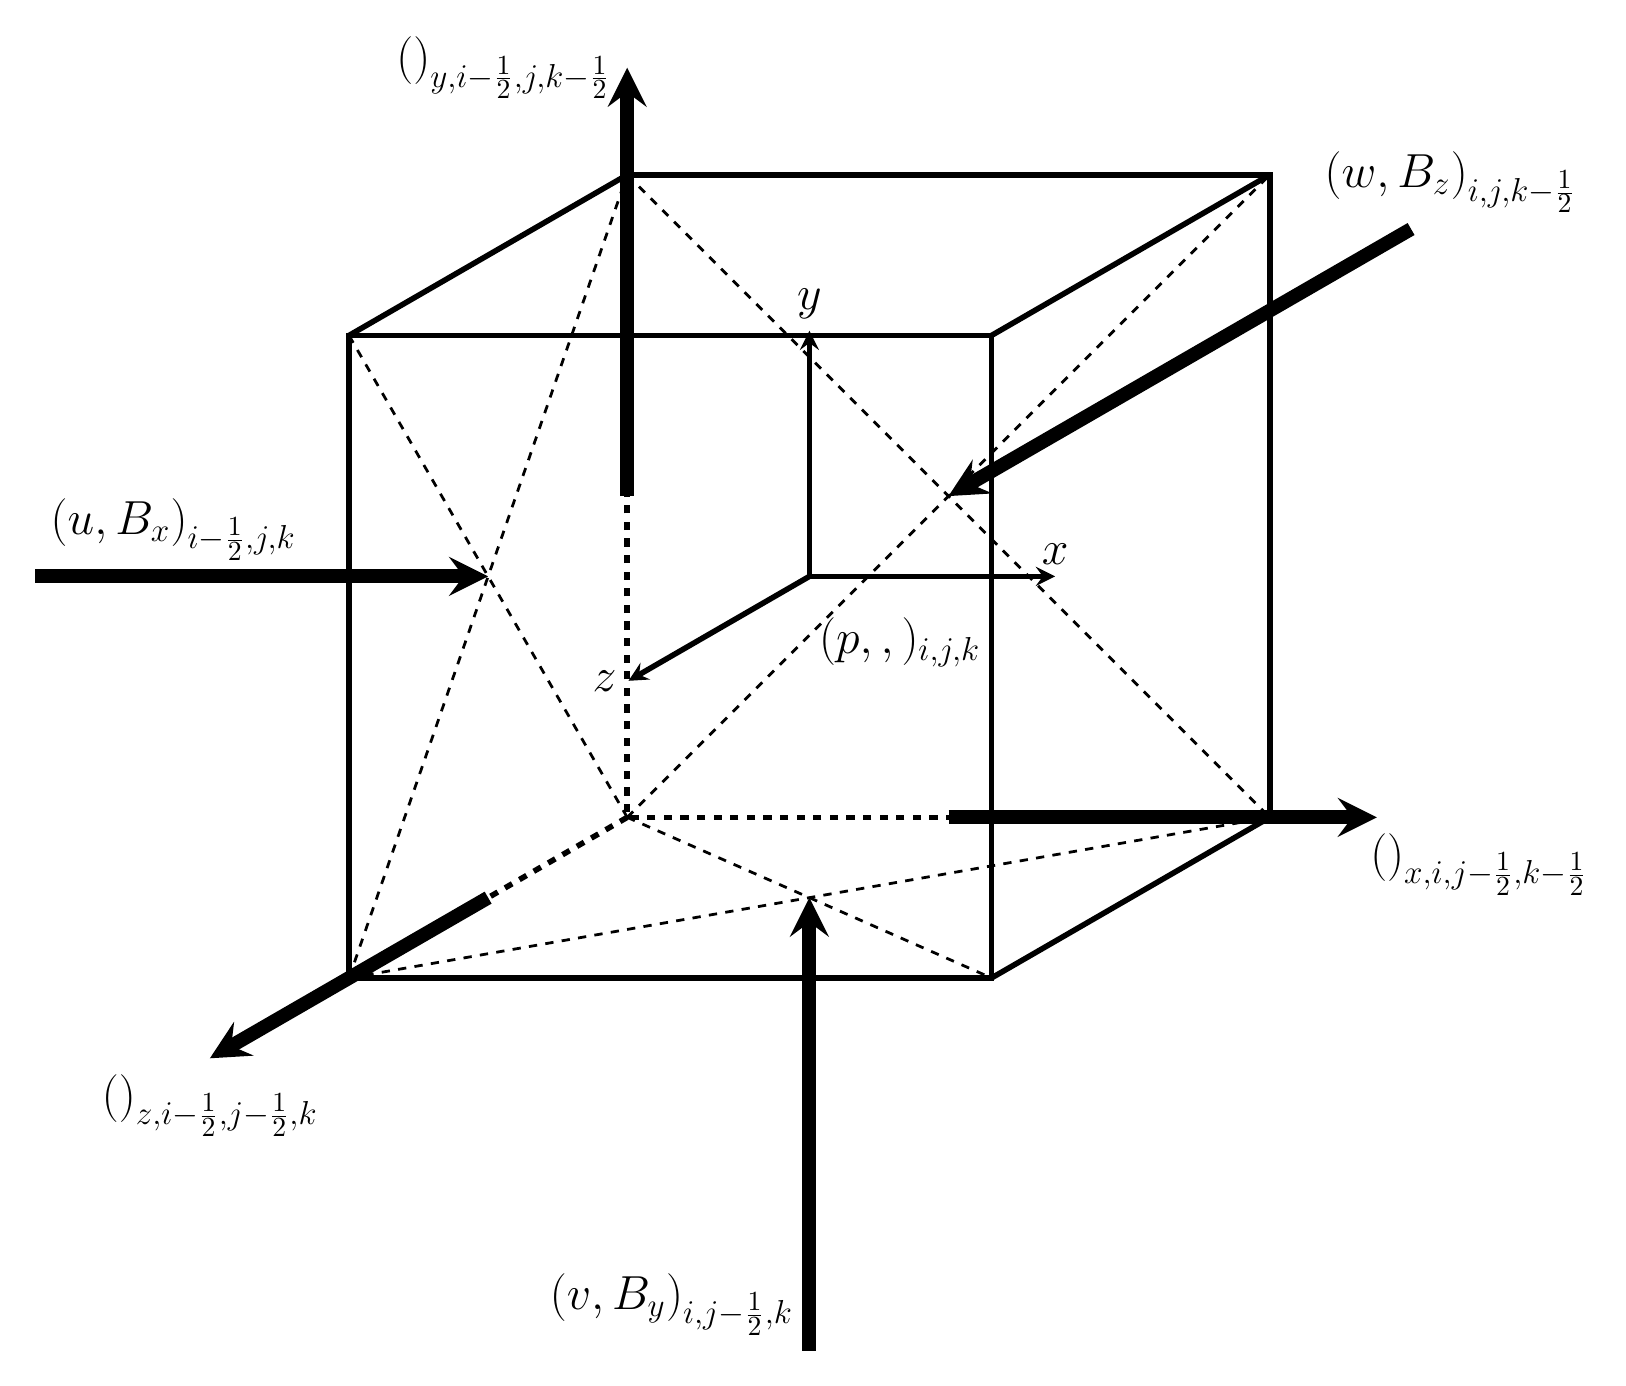
\begin{tikzpicture}[scale=\s]
% SIZES: \tiny \scriptsize \footnotesize \small \normalsize \large \Large \LARGE \huge \Huge
\tikzstyle{every node}=[font=\LARGE]

% Back face lines
\draw[line width=\wSquare,dashed] (\OR+\dx,\OR) -- ++ (-\dx,0) -- ++ (0,\dy);
\draw[line width=\wSquare]        (\OR+\dx,\OR) -- ++	(0,\dy) -- ++ (-\dx,0);
% Front face lines
\draw[line width=\wSquare] (-{\cosL}+\OR,-{\sinL}+\OR) -- ++ (\dx,0) -- ++ (0,\dy);
\draw[line width=\wSquare] (-{\cosL}+\OR,-{\sinL}+\OR) -- ++ (0,\dy) -- ++ (\dx,0);

% % Back face circles
% \draw[fill,line width=\w] (\OR,\OR) circle [radius=\ra];
% \draw[fill,line width=\w] (\OR+\dx,\OR) circle [radius=\ra];
% \draw[fill,line width=\w] (\OR+\dx,\OR+\dy) circle [radius=\ra];
% \draw[fill,line width=\w] (\OR,\OR+\dy) circle [radius=\ra];
% % Front face circles
% \draw[fill,line width=\wSquare] (-{\cosL}+\OR,-{\sinL}+\OR) circle [radius=\ra];
% \draw[fill,line width=\wSquare] (-{\cosL}+\OR+\dx,-{\sinL}+\OR) circle [radius=\ra];
% \draw[fill,line width=\wSquare] (-{\cosL}+\OR+\dx,-{\sinL}+\OR+\dy) circle [radius=\ra];
% \draw[fill,line width=\wSquare] (-{\cosL}+\OR,-{\sinL}+\OR+\dy) circle [radius=\ra];

% Connecting lines
\draw[line width=\wSquare,dashed] (\OR,\OR)         -- ++({-\cosL},{-\sinL});
\draw[line width=\wSquare]        (\OR+\dx,\OR)     -- ++({-\cosL},{-\sinL});
\draw[line width=\wSquare]        (\OR+\dx,\OR+\dy) -- ++({-\cosL},{-\sinL});
\draw[line width=\wSquare]        (\OR,\OR+\dy)     -- ++({-\cosL},{-\sinL});

% Criss-cross lines (Sergey's request)
\draw[line width=\wCrissCross,dashed] (\OR,\OR) -- ++(\dx,\dy);
\draw[line width=\wCrissCross,dashed] (\OR,\OR) -- ++(-{\cosL}+\dx,-{\sinL});
\draw[line width=\wCrissCross,dashed] (\OR,\OR) -- ++(-{\cosL},-{\sinL}+\dy);

\draw[line width=\wCrissCross,dashed] (-{\cosL}+\OR,-{\sinL}+\OR) -- ++({\dx+\cosL},{\sinL});
\draw[line width=\wCrissCross,dashed] (-{\cosL}+\OR,-{\sinL}+\OR) -- ++({\cosL},{\dy+\sinL});
\draw[line width=\wCrissCross,dashed] (\OR,\OR+\dy) -- ++(\dx,-\dy);

% E/J Field
\draw[\arrR,anchor=east,line width=\wArr]
(\OR+\dx/2,\OR) -- ++(\dx/1.5,0) node[right=1.3,anchor=north]
{$(\CURL \B)_{x,i,j-\frac{1}{2},k-\frac{1}{2}}$};
\draw[\arrR,anchor=east,line width=\wArr]
(\OR,\OR+\dy/2) -- ++(0,\dy/1.5) node[anchor=east]
{$(\CURL \B)_{y,i-\frac{1}{2},j,k-\frac{1}{2}}$};
\draw[\arrR,anchor=east,line width=\wArr]
({\OR-\cosL/2},{\OR-\sinL/2}) -- ++({-\cosL},{-\sinL}) node[anchor=north]
{$(\CURL \B)_{z,i-\frac{1}{2},j-\frac{1}{2},k}$};

% \draw[\arrR,anchor=east,line width=\w]  (\OR+\dx/2,\OR) -- ++(\dx/1.5,0) node[anchor=west]{$(\CURL \B)_x, (\U \times \B)_x$};
% \draw[\arrR,anchor=east,line width=\w]  (\OR,\OR+\dy/2) -- ++(0,\dy/1.5) node[anchor=east]{$(\CURL \B)_y, (\U \times \mathbf{\text{B}})_y$};
% \draw[\arrR,anchor=east,line width=\w]  ({\OR-\cosL/2},{\OR-\sinL/2}) -- ++({-\cosL/1.3},{-\sinL/1.3}) node[anchor=east]{$(\CURL \B)_z, (\U \times \B)_z$};

% u,v,w
\draw[line width=\wArr,\arrL] (\CCx-\dx/2,\CCy)
-- ++(-\arrowL,0) node[anchor=south west]
{$(u,B_x)_{i-\frac{1}{2},j,k}$};%x
\draw[line width=\wArr,\arrL] (\CCx,\CCy-\dy/2)
-- ++(0,-\arrowL) node[anchor=south east]
{$(v,B_y)_{i,j-\frac{1}{2},k}$};%y
\draw[line width=\wArr,\arrL] (\OR+\dx/2,\OR+\dy/2)
-- ++({\cosL*\arrowLZ},{\sinL*\arrowLZ}) node[left=-0.5,anchor=south]
{$(w,B_z)_{i,j,k-\frac{1}{2}}$};%z

% Coordinate system
% \draw[line width=\w,\arrR] (\OR+\COx,\OR+\COy) -- ++(0,\coordL) node[anchor=south]{$y$};
% \draw[line width=\w,\arrR] (\OR+\COx,\OR+\COy) -- ++(\coordL,0) node[anchor=north]{$x$};
% \draw[line width=\w,\arrR] (\OR+\COx,\OR+\COy) -- ++({-\cosL*\coordL},{-\sinL*\coordL}) node[anchor=east]{$z$};

% B system
\draw[line width=\wCoord,\arrR]
	(\CCx,\CCy) -- ++
	(0,\coordL) node[anchor=south]{$y$};
\draw[line width=\wCoord,\arrR]
	(\CCx,\CCy) -- ++
	(\coordL,0) node[anchor=south]{$x$};
\draw[line width=\wCoord,\arrR]
	(\CCx,\CCy) -- ++
	({-\cosL*\coordL},{-\sinL*\coordL}) node[anchor=east]{$z$};

% Pressure circle
% \draw [fill] (\CCx,\CCy) circle [radius=0.03];
\draw (\CCx,\CCy) node[below=0.4,anchor=north west]
{$(p, \DEL \DOT \U, \DEL \DOT \B)_{i,j,k}$};

\end{tikzpicture}



\end{document}